% cpu/cpu.tex

\chapter{Hardware and its Habits}
\label{chp:Hardware and its Habits}

\QuickQuizChapter{chp:Hardware and its Habits}

Most people have an intuitive understanding that passing messages between
systems is considerably more expensive than performing simple calculations
within the confines of a single system.
However, it is not always so clear that communicating among threads within
the confines of a single shared-memory system can also be quite expensive.
This chapter therefore looks the cost of synchronization and communication
within a shared-memory system.
This chapter merely scratches the surface of shared-memory parallel
hardware design; readers desiring more detail would do well to start
with a recent edition of
Hennessy's and Patterson's classic text~\cite{Hennessy95a}.

\QuickQuiz{}
	Why should parallel programmers bother learning low-level
	properties of the hardware?
	Wouldn't it be easier, better, and more general to remain at
	a higher level of abstraction?
\QuickQuizAnswer{
	It might well be easier to ignore the detailed properties of
	the hardware, but in most cases it would be quite foolish
	to do so.
	If you accept that the only purpose of parallelism is to
	increase performance, and if you further accept that
	performance depends on detailed properties of the hardware,
	then it logically follows that parallel programmers are going
	to need to know at least a few hardware properties.

	This is the case in most engineering disciplines.
	Would \emph{you} want to use a bridge designed by an
	engineer who did not understand the properties of
	the concrete and steel making up that bridge?
	If not, why would you expect a parallel programmer to be
	able to develop competent parallel software without at least
	\emph{some} understanding of the underlying hardware?
} \QuickQuizEnd

% cpu/overview.tex

\section{Overview}
\label{sec:cpu:Overview}

Careless reading of computer-system specification sheets might lead one
to believe that CPU performance is a footrace on a clear track, as
illustrated in Figure~\ref{fig:cpu:CPU Performance at its Best},
where the race always goes to the swiftest.

\begin{figure}[htb]
\begin{center}
\resizebox{3in}{!}{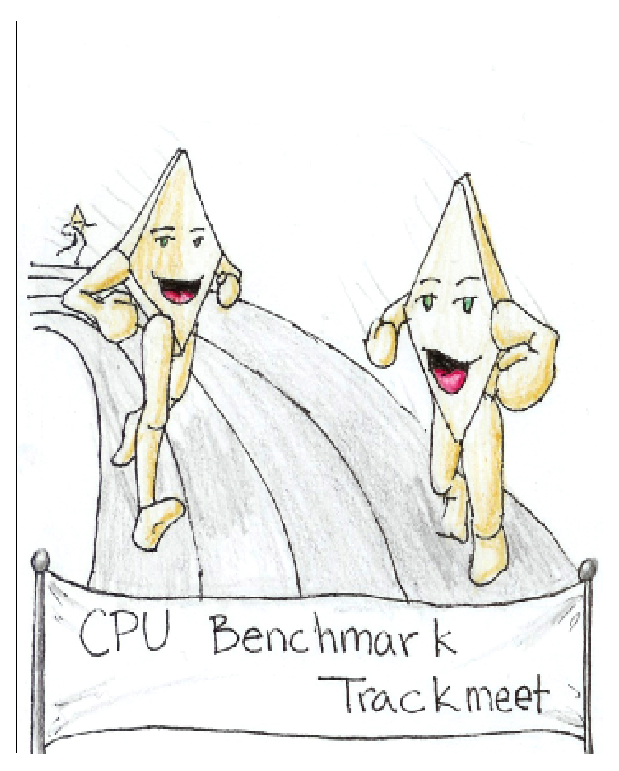
\includegraphics{cartoons/trackmeet}}
\end{center}
\caption{CPU Performance at its Best}
\ContributedBy{Figure}{fig:cpu:CPU Performance at its Best}{Melissa McKenney}
\end{figure}

Although there are a few CPU-bound benchmarks that approach the ideal
shown in Figure~\ref{fig:cpu:CPU Performance at its Best},
the typical program more closely resembles an obstacle course than
a race track.
This is because the internal architecture of CPUs has changed dramatically
over the past few decades, courtesy of Moore's Law.
These changes are described in the following sections.

\subsection{Pipelined CPUs}
\label{sec:cpu:Pipelined CPUs}

\begin{figure}[htb]
\begin{center}
\resizebox{3in}{!}{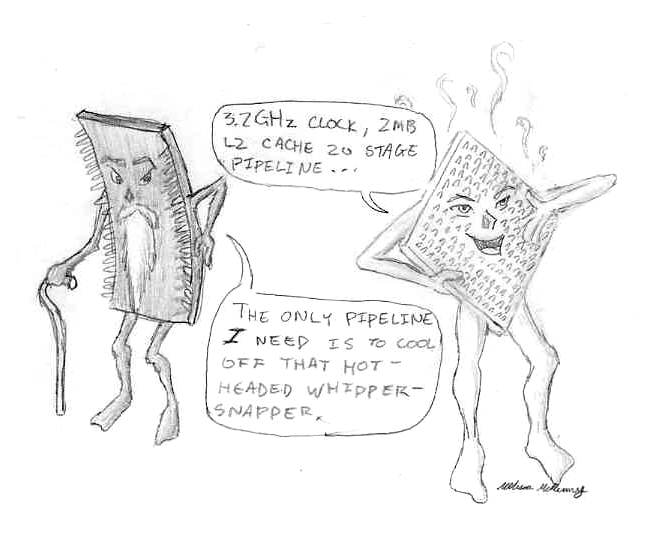
\includegraphics{cartoons/whippersnapper}}
\end{center}
\caption{CPUs Old and New}
\ContributedBy{Figure}{fig:cpu:CPUs Old and New}{Melissa McKenney}
\end{figure}

In the early 1980s, the typical microprocessor fetched an instruction,
decoded it, and executed it, typically taking \emph{at least} three
clock cycles to complete one instruction before proceeding to the next.
In contrast, the CPU of the late 1990s and early 2000s will be executing
many instructions simultaneously, using a deep ``pipeline'' to control
the flow of instructions internally to the CPU, this difference being
illustrated by Figure~\ref{fig:cpu:CPUs Old and New}.

Achieving full performance with a CPU having a long pipeline requires
highly predictable control flow through the program.
Suitable control flow can be provided by a program that executes primarily
in tight loops, for example, programs doing arithmetic on large matrices
or vectors.
The CPU can then correctly predict that the branch at the end of the loop
will be taken in almost all cases.
In such programs, the pipeline can be kept full and the CPU can execute
at full speed.

\begin{figure}[htb]
\begin{center}
\resizebox{3in}{!}{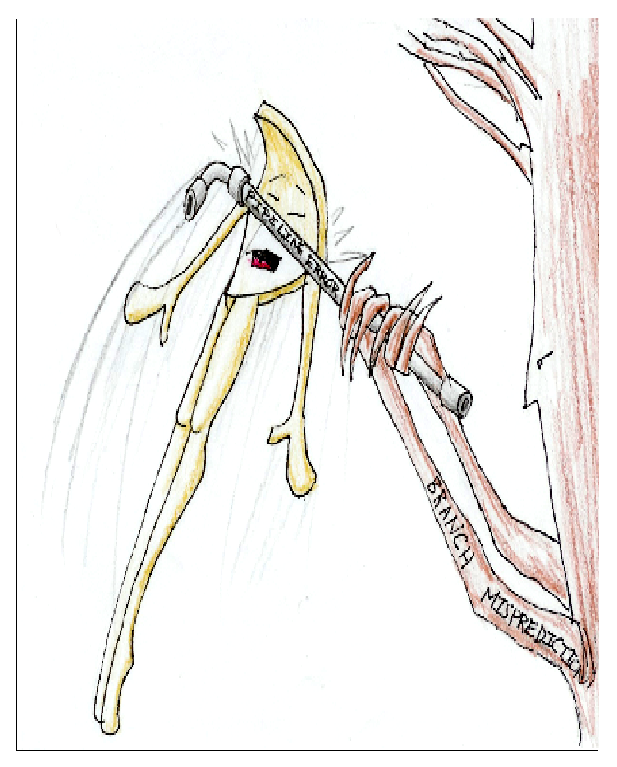
\includegraphics{cartoons/pipeline}}
\end{center}
\caption{CPU Meets a Pipeline Flush}
\ContributedBy{Figure}{fig:cpu:CPU Meets a Pipeline Flush}{Melissa McKenney}
\end{figure}

If, on the other hand, the program has many loops with small loop counts,
or if the program is object oriented with many virtual objects that
can reference many different real objects, all with different implementations
for frequently invoked member functions, then it is difficult or even
impossible for the CPU to predict where a given branch might lead.
The CPU must then either stall waiting for execution to proceed far enough
to know for certain where the branch will lead, or guess --- and, in the
face of programs with unpredictable control flow, frequently guess wrong.
In either case, the pipeline will empty and have to be refilled, leading
to stalls that can drastically reduce performance,
as fancifully depicted in Figure~\ref{fig:cpu:CPU Meets a Pipeline Flush}.

Unfortunately, pipeline flushes are not the only hazards in the obstacle
course that modern CPUs must run.
The next section covers the hazards of referencing memory.

\subsection{Memory References}
\label{sec:cpu:Memory References}

In the 1980s, it often took less time for a microprocessor to load a value
from memory than it did to execute an instruction.
In 2006, a microprocessor might be capable of executing hundreds or even
thousands of instructions in the time required to access memory.
This disparity is due to the fact that Moore's Law has increased CPU
performance at a much greater rate than it has increased memory
performance, in part due to the rate at which memory sizes have
grown.
For example, a typical 1970s minicomputer might have 4KB (yes, kilobytes,
not megabytes, let alone gigabytes) of main memory, with single-cycle access.
In 2008, CPU designers still can construct a 4KB memory with single-cycle
access, even on systems with multi-GHz clock frequencies.
And in fact they frequently do construct such memories, but they now
call them ``level-0 caches''.

Although the large caches found on modern microprocessors can do quite
a bit to help combat memory-access latencies,
these caches require highly predictable data-access patterns to
successfully hide memory latencies.
Unfortunately, common operations, such as traversing a linked list,
have extremely unpredictable memory-access patterns --- after all,
if the pattern was predictable, us software types would not bother
with the pointers, right?

\begin{figure}[htb]
\begin{center}
\resizebox{3in}{!}{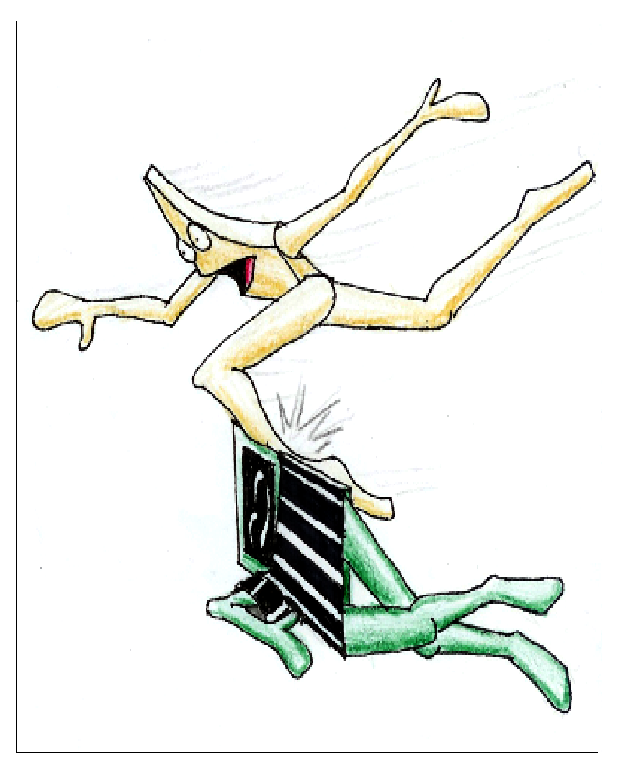
\includegraphics{cartoons/ref}}
\end{center}
\caption{CPU Meets a Memory Reference}
\ContributedBy{Figure}{fig:cpu:CPU Meets a Memory Reference}{Melissa McKenney}
\end{figure}

Therefore, as shown in
Figure~\ref{fig:cpu:CPU Meets a Memory Reference},
memory references are often severe obstacles for modern CPUs.

Thus far, we have only been considering obstacles that can arise during
a given CPU's execution of single-threaded code.
Multi-threading presents additional obstacles to the CPU, as
described in the following sections.

\subsection{Atomic Operations}
\label{sec:cpu:Atomic Operations}

One such obstacle is atomic operations.
The whole idea of an atomic operation in some sense conflicts with
the piece-at-a-time assembly-line operation of a CPU pipeline.
To hardware designers' credit, modern CPUs use a number of extremely clever
tricks to make such operations \emph{look} atomic even though they
are in fact being executed piece-at-a-time, but even so, there are
cases where the pipeline must be delayed or even flushed in order to
permit a given atomic operation to complete correctly.

\begin{figure}[htb]
\begin{center}
\resizebox{3in}{!}{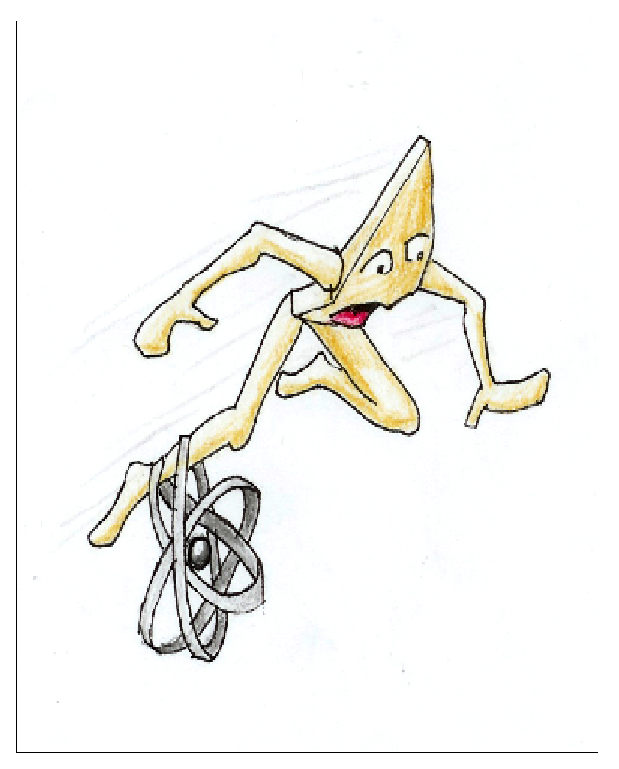
\includegraphics{cartoons/atomic}}
\end{center}
\caption{CPU Meets an Atomic Operation}
\ContributedBy{Figure}{fig:cpu:CPU Meets an Atomic Operation}{Melissa McKenney}
\end{figure}

The resulting effect on performance is depicted in
Figure~\ref{fig:cpu:CPU Meets an Atomic Operation}.

Unfortunately, atomic operations usually apply only to single elements
of data.
Because many parallel algorithms require that ordering constraints
be maintained between updates of multiple data elements, most CPUs
provide memory barriers.
These memory barriers also serve as performance-sapping obstacles,
as described in the next section.

\QuickQuiz{}
	What types of machines would allow atomic operations on
	multiple data elements?
\QuickQuizAnswer{
	One answer to this question is that it is often possible to
	pack multiple elements of data into a single machine word,
	which can then be manipulated atomically.

	A more trendy answer would be machines supporting transactional
	memory~\cite{DBLomet1977SIGSOFT}.
	However, such machines are still (as of 2008) research
	curiosities.
	The jury is still out on the applicability of transactional
	memory~\cite{McKenney2007PLOSTM,DonaldEPorter2007TRANSACT,
	ChistopherJRossbach2007a}.
} \QuickQuizEnd

\subsection{Memory Barriers}
\label{sec:cpu:Memory Barriers}

Memory barriers will be considered in more detail in
Section~\ref{sec:advsync:Memory Barriers} and
Appendix~\ref{chp:app:whymb:Why Memory Barriers?}.
In the meantime, consider the following simple lock-based critical
section:

\vspace{5pt}
\begin{minipage}[t]{\columnwidth}
\small
\begin{verbatim}
  1 spin_lock(&mylock);
  2 a = a + 1;
  3 spin_unlock(&mylock);
\end{verbatim}
\end{minipage}
\vspace{5pt}

\begin{figure}[tb]
\begin{center}
\resizebox{3in}{!}{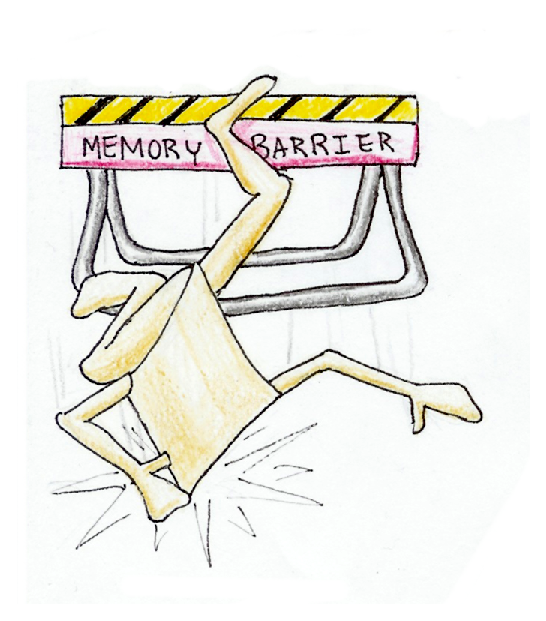
\includegraphics{cartoons/barrier}}
\end{center}
\caption{CPU Meets a Memory Barrier}
\ContributedBy{Figure}{fig:cpu:CPU Meets a Memory Barrier}{Melissa McKenney}
\end{figure}

If the CPU were not constrained to execute these statements in the
order shown, the effect would be that the variable ``a'' would be
incremented without the protection of ``mylock'', which would certainly
defeat the purpose of acquiring it.
To prevent such destructive reordering, locking primitives contain
either explicit or implicit memory barriers.
Because the whole purpose of these memory barriers is to prevent reorderings
that the CPU would otherwise undertake in order to increase performance,
memory barriers almost always reduce performance, as depicted in
Figure~\ref{fig:cpu:CPU Meets a Memory Barrier}.

\subsection{Cache Misses}
\label{sec:cpu:Cache Misses}

\begin{figure}[htb]
\begin{center}
\resizebox{3in}{!}{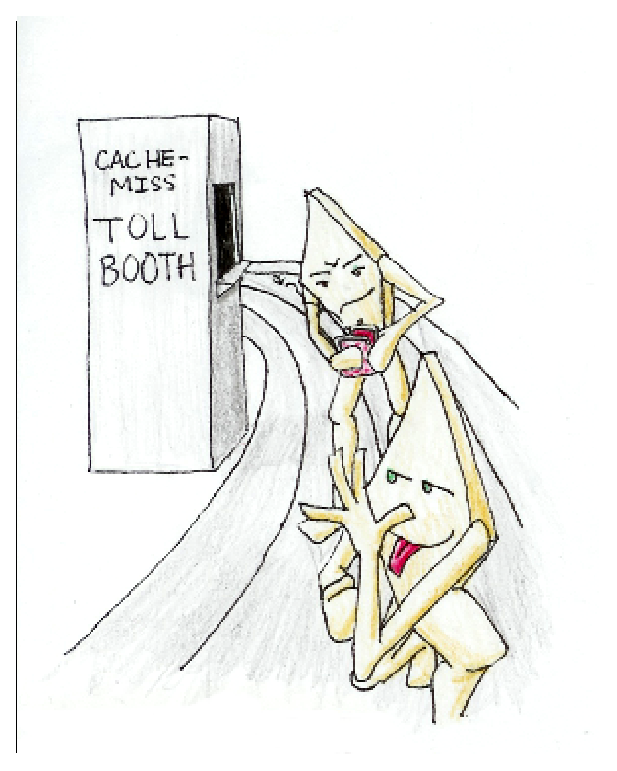
\includegraphics{cartoons/tollbooth}}
\end{center}
\caption{CPU Meets a Cache Miss}
\ContributedBy{Figure}{fig:cpu:CPU Meets a Cache Miss}{Melissa McKenney}
\end{figure}

An additional multi-threading obstacle to CPU performance is
the ``cache miss''.
As noted earlier, modern CPUs sport large caches in order to reduce the
performance penalty that would otherwise be incurred due to slow memory
latencies.
However, these caches are actually counter-productive for variables that
are frequently shared among CPUs.
This is because when a given CPU wishes to modify the variable, it is
most likely the case that some other CPU has modified it recently.
In this case, the variable will be in that other CPU's cache, but not
in this CPU's cache, which will therefore incur an expensive cache miss
(see Section~\ref{sec:app:whymb:Cache Structure} for more detail).
Such cache misses form a major obstacle to CPU performance, as shown
in Figure~\ref{fig:cpu:CPU Meets a Cache Miss}.

\subsection{I/O Operations}
\label{sec:cpu:I/O Operations}

\begin{figure}[htb]
\begin{center}
\resizebox{3in}{!}{\includegraphics{cartoons/PhoneBooth}}
\end{center}
\caption{CPU Waits for I/O Completion}
\ContributedBy{Figure}{fig:cpu:CPU Waits for I/O Completion}{Melissa McKenney}
\end{figure}

A cache miss can be thought of as a CPU-to-CPU I/O operation, and as
such is one of the cheapest I/O operations available.
I/O operations involving networking, mass storage, or (worse yet) human
beings pose much greater obstacles than the internal obstacles called
out in the prior sections,
as illustrated by
Figure~\ref{fig:cpu:CPU Waits for I/O Completion}.

This is one of the differences between shared-memory and distributed-system
parallelism: shared-memory parallel programs must normally deal with no
obstacle worse than a cache miss, while a distributed parallel program
will typically incur the larger network communication latencies.
In both cases, the relevant latencies can be thought of as a cost of
communication---a cost that would be absent in a sequential program.
Therefore, the ratio between the overhead of the communication to
that of the actual work being performed is a key design parameter.
A major goal of parallel design is to reduce this ratio as needed to
achieve the relevant performance and scalability goals.

Of course, it is one thing to say that a given operation is an obstacle,
and quite another to show that the operation is a \emph{significant}
obstacle.
This distinction is discussed in the following sections.

% cpu/overheads.tex

\section{Overheads}
\label{sec:cpu:Overheads}

This section presents actual overheads of the obstacles to performance
listed out in the previous section.
However, it is first necessary to get a rough view of hardware system
architecture, which is the subject of the next section.

\subsection{Hardware System Architecture}
\label{sec:cpu:Hardware System Architecture}

\begin{figure}[tb]
\begin{center}
\resizebox{3in}{!}{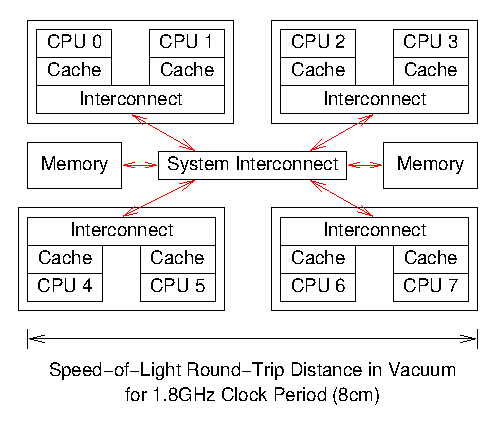
\includegraphics{cpu/SystemArch}}
\end{center}
\caption{System Hardware Architecture}
\label{fig:cpu:System Hardware Architecture}
\end{figure}

Figure~\ref{fig:cpu:System Hardware Architecture}
shows a rough schematic of an eight-core computer system.
Each die has a pair of CPU cores, each with its cache, as well as an
interconnect allowing the pair of CPUs to communicate with each other.
The system interconnect in the middle of the diagram allows the
four dies to communicate, and also connects them to main memory.

Data moves through this system in units of ``cache lines'', which
are power-of-two fixed-size aligned blocks of memory, usually ranging
from 32 to 256 bytes in size.
When a CPU loads a variable from memory to one of its registers, it must
first load the cacheline containing that variable into its cache.
Similarly, when a CPU stores a value from one of its registers into
memory, it must also load the cacheline containing that variable into
its cache, but must also ensure that no other CPU has a copy of that
cacheline.

For example, if CPU~0 were to perform a compare-and-swap (CAS) operation on a
variable whose cacheline resided in CPU~7's cache, the following
over-simplified sequence of events might ensue:

\begin{enumerate}
\item	CPU~0 checks its local cache, and does not find the cacheline.
\item	The request is forwarded to CPU~0's and 1's interconnect,
	which checks CPU~1's local cache, and does not find the cacheline.
\item	The request is forwarded to the system interconnect, which
	checks with the other three dies, learning that the cacheline
	is held by the die containing CPU~6 and 7.
\item	The request is forwarded to CPU~6's and 7's interconnect, which
	checks both CPUs' caches, finding the value in CPU~7's cache.
\item	CPU~7 forwards the cacheline to its interconnect, and also
	flushes the cacheline from its cache.
\item	CPU~6's and 7's interconnect forwards the cacheline to the
	system interconnect.
\item	The system interconnect forwards the cacheline to CPU~0's and 1's
	interconnect.
\item	CPU~0's and 1's interconnect forwards the cacheline to CPU~0's
	cache.
\item	CPU~0 can now perform the CAS operation on the value in its cache.
\end{enumerate}

\QuickQuiz{}
	This is a \emph{simplified} sequence of events?
	How could it \emph{possibly} be any more complex?
\QuickQuizAnswer{
	This sequence ignored a number of possible complications,
	including:

	\begin{enumerate}
	\item	Other CPUs might be concurrently attempting to perform
		CAS operations involving this same cacheline.
	\item	The cacheline might have been replicated read-only in
		several CPUs' caches, in which case, it would need to
		be flushed from their caches.
	\item	CPU~7 might have been operating on the cache line when
		the request for it arrived, in which case CPU~7 would
		need to hold of the request until its own operation
		completed.
	\item	CPU~7 might have ejected the cacheline from its cache
		(for example, in order to make room for other data),
		so that by the time that the request arrived, the
		cacheline was on its way to memory.
	\item	A correctable error might have occurred in the cacheline,
		which would then need to be corrected at some point before
		the data was used.
	\end{enumerate}

	Production-quality cache-coherence mechanisms are extremely
	complicated due to these sorts of considerations.

} \QuickQuizEnd

\QuickQuiz{}
	Why is it necessary to flush the cacheline from CPU~7's cache?
\QuickQuizAnswer{
	If the cacheline was not flushed from CPU~7's cache, then
	CPUs~0 and 7 might have different values for the same set
	of variables in the cacheline.
	This sort of incoherence would greatly complicate parallel
	software, and so hardware architects have been convinced to
	avoid it.
} \QuickQuizEnd

\subsection{Costs of Operations}
\label{sec:cpu:Costs of Operations}

\begin{table}
\centering
\begin{tabular}{l||r|r}
	Operation		& Cost (ns) 	& Ratio \\
	\hline
	\hline
	Clock period		&           0.6	&           1.0 \\
	\hline
	Best-case CAS		&          37.9	&          63.2 \\
	\hline
	Best-case lock		&          65.6	&         109.3\\
	\hline
	Single cache miss	&         139.5	&         232.5 \\
	\hline
	CAS cache miss		&         306.0	&         510.0 \\
	\hline
	Comms Fabric		&       3,000	&       5,000 \\
	\hline
	Global Comms		& 130,000,000	& 216,000,000 \\
\end{tabular}
\caption{Performance of Synchronization Mechanisms on 4-CPU 1.8GHz AMD Opteron 844 System}
\label{tab:cpu:Performance of Synchronization Mechanisms on 4-CPU 1.8GHz AMD Opteron 844 System}
\end{table}

The overheads of some common operations important to parallel programs are
displayed in
Table~\ref{tab:cpu:Performance of Synchronization Mechanisms on 4-CPU 1.8GHz AMD Opteron 844 System}.
This system's clock period rounds to 0.6ns.
Although it is not unusual for modern microprocessors to be able to retire
multiple instructions per clock period, the operations will be normalized
to a full clock period in the third column, labeled ``Ratio''.
The first thing to note about this table is the large values of many of
the ratios.

The best-case CAS operation consumes almost forty
nanoseconds, a duration more than sixty times that of the clock period.
Here, ``best case'' means that the same CPU now performing the CAS operation
on a given variable was the last CPU to operate on this variable, so
that the corresponding cache line is already held in that CPU's cache,
Similarly, the best-case lock operation (a ``round trip'' pair consisting
of a lock acquisition followed by a lock release) consumes more than
sixty nanosecond, or more than one hundred lock cycles.
Again, ``best case'' means that the data structure representing the
lock is already in the cache belonging to the CPU acquiring and releasing
the lock.
The lock operation is more expensive than CAS because it requires two
atomic operations on the lock data structure.

An operation that misses the cache consumes almost one hundred and forty
nanoseconds, or more than two hundred clock cycles.
A CAS operation, which must look at the old value of the variable as
well as store a new value, consumes over three hundred nanoseconds, or
more than five hundred clock cycles.
Think about this a bit.
In the time required to do \emph{one} CAS operation, the CPU could have
executed more than \emph{five hundred} normal instructions.
This should demonstrate the limitations of fine-grained locking.

\QuickQuiz{}
	Surely the hardware designers could be persuaded to improve
	this situation!
	Why have they been content with such abysmal performance
	for these single-instruction operations?
\QuickQuizAnswer{
	The hardware designers \emph{have} been working on this
	problem, and have consulted with no less a luminary than
	the physicist Stephen Hawking.
	Hawking's observation was that the hardware designers have
	two basic problems~\cite{BryanGardiner2007}:

	\begin{enumerate}
	\item	the finite speed of light, and
	\item	the atomic nature of matter.
	\end{enumerate}

\begin{table}
\centering
\begin{tabular}{l||r|r}
	Operation		& Cost (ns) 	& Ratio \\
	\hline
	\hline
	Clock period		&           0.4	&           1.0 \\
	\hline
	``Best-case'' CAS	&          12.2	&          33.8 \\
	\hline
	Best-case lock		&          25.6	&          71.2 \\
	\hline
	Single cache miss	&          12.9	&          35.8 \\
	\hline
	CAS cache miss		&           7.0	&          19.4 \\
	\hline
	Off-Core		&		&		\\
	\hline
	Single cache miss	&          31.2	&          86.6 \\
	\hline
	CAS cache miss		&          31.2	&          86.5 \\
	\hline
	Off-Socket		&		&		\\
	\hline
	Single cache miss	&          92.4	&         256.7 \\
	\hline
	CAS cache miss		&          95.9	&         266.4 \\
	\hline
	Comms Fabric		&       4,500	&       7,500 \\
	\hline
	Global Comms		& 195,000,000	& 324,000,000 \\
\end{tabular}
\caption{Performance of Synchronization Mechanisms on 16-CPU 2.8GHz Intel X5550 (Nehalem) System}
\label{tab:cpu:Performance of Synchronization Mechanisms on 16-CPU 2.8GHz Intel X5550 (Nehalem) System}
\end{table}

	The first problem limits raw speed, and the second limits
	miniaturization, which in turn limits frequency.
	And even this sidesteps the power-consumption issue that
	is currently holding production frequencies to well below
	10 GHz.

	Nevertheless, some progress is being made, as may be seen
	by comparing
	Table~\ref{tab:cpu:Performance of Synchronization Mechanisms on 16-CPU 2.8GHz Intel X5550 (Nehalem) System}
	with
	Table~\ref{tab:cpu:Performance of Synchronization Mechanisms on 4-CPU 1.8GHz AMD Opteron 844 System}
	on
	page~\ref{tab:cpu:Performance of Synchronization Mechanisms on 4-CPU 1.8GHz AMD Opteron 844 System}.
	Integration of hardware threads in a single core and multiple
	cores on a die have improved latencies greatly, at least within the
	confines of a single core or single die.
	There has been some improvement in overall system latency,
	but only by about a factor of two.
	Unfortunately, neither the speed of light nor the atomic nature
	of matter has changed much in the past few years.

	Section~\ref{sec:cpu:Hardware Free Lunch?}
	looks at what else hardware designers might be
	able to do to ease the plight of parallel programmers.
} \QuickQuizEnd

I/O operations are even more expensive.
A high performance (and expensive!) communications fabric, such as
InfiniBand or any number of proprietary interconnects, has a latency
of roughly three microseconds, during which time five \emph{thousand}
instructions might have been executed.
Standards-based communications networks often require some sort of
protocol processing, which further increases the latency.
Of course, geographic distance also increases latency, with the
theoretical speed-of-light latency around the world coming to
roughly 130 \emph{milliseconds}, or more than 200 million clock
cycles.

\QuickQuiz{}
	These numbers are insanely large!
	How can I possibly get my head around them?
\QuickQuizAnswer{
	Get a roll of toilet paper.
	In the USA, each roll will normally have somewhere around 350-500
	sheets.
	Tear off one sheet to represent a single clock cycle, setting it aside.
	Now unroll the rest of the roll.

	The resulting pile of toilet paper will likely represent a single
	CAS cache miss.

	For the more-expensive inter-system communications latencies,
	use several rolls (or multiple cases) of toilet paper to represent
	the communications latency.

	Important safety tip: make sure to account for the needs of
	those you live with when appropriating toilet paper!
} \QuickQuizEnd

